\chapter{Metody numeryczne}

Materiały teoretyczne z metod numerycznych zostały opracowane na podstawie \href{https://www.mimuw.edu.pl/~przykry/mn/moon-handouts.pdf}{slajdów Piotra Krzyżanowskiego}.

\section*{Podstawa programowa}
\begin{enumerate}
    \item Algorytmy \textbf{rozkładu macierzy} i ich zastosowania.
    \item \textbf{Uwarunkowanie i numeryczna poprawność}.
    \item \textbf{Metody iteracyjne} rozwiązywania układów równań liniowych i nieliniowych.
    \item \textbf{Interpolacja wielomianowa}.
    \item \textbf{Aproksymacja jednostajna} oraz w przestrzeniach unitarnych.
    \item Metody numeryczne \textbf{całkowania}.
\end{enumerate}

\section{Algorytmy rozkładu macierzy}
\subsection{Normy}
Warto jest orientować się w normach wektorowych
\begin{itemize}
    \item $\|x\|_1 = \sum_{i=1}^{N}|x_i|$, $\ \ \|x\|_2 = \sqrt{\sum_{i=1}^N|x_i|^2}$, $\ \ \|x\|_p = \left(\sum_{i=1}^N|x_i|^p \right)^{1/p}$
    \item $\|x\|_{\infty} = \max_i|x_i|$, $\ \ \|x\|_{\infty}\leq \|x\|_1\leq N\|x\|_{\infty}$
    \item $\|x\|_2 \leq \|x\|_1\leq \sqrt{N}\|x\|_2$, $\ \ \|x\|_{\infty} \leq \|x\|_2 \leq \sqrt{N}\|x\|_{\infty}$
\end{itemize}
oraz normach macierzowych
\begin{itemize}
    \item $\|Ax\|\leq \|A\|\cdot \|x\|$, $\ \ \|AB\| \leq \|A\|\cdot\|B\|$, $\ \ \|I\|=1$
    \item $\|A\|_1=\max_j\sum_i|a_{ij}|$ (kolumnowa)
    \item $\|A\|_{\infty}=\max_i\sum_j|a_{ij}|$ (wierszowa)
    \item $\|A\|_2 = max\{\sqrt{\mu} : \mu \mbox{ to w.wł } A^TA\} = \sqrt{\rho(A^TA)}$ (spektralna)
\end{itemize}

\subsection{Ortogonalność}
Macierz $Q\in \RR^{n,n}$ nazywamy \textbf{ortogonalną}, jeśli
$$
Q^TQ=I,
$$
czyli kolumny $Q$ są wzajemnie prostopadłe, a ich norma euklidesowa jest równa $1$. \purple{\textbf{UWAGA!}}: na numerkach zazwyczaj ortogonalność to znana z GALu ortonormalność (stąd uwaga o normie euklidesowej).

\subsection{Przydatne typy macierzy}
\textbf{Macierz górno(dolno)trójkątna} to macierz kwadratowa, która ma elementy niezerowe jedynie na diagonali oraz ponad (poniżej) niej. 
$$
A=\begin{bmatrix}
    a_{1,1} & a_{1,2} & a_{1,3} & \dots & a_{1,n} \\
    0 & a_{2,2} & a_{2,3} & \dots & a_{2,n} \\
    0 & 0 & a_{3,3} & \dots & a_{3,n} \\ 
    \dots & \dots & \dots & \dots & \dots \\
    0 & 0 & 0 & \dots & a_{n,n}
\end{bmatrix} \quad\mbox{ jest macierzą górnotrójkątną}.
$$
Wyznacznik macierzy trójkątnej równy jest iloczynowi elementów na jej diagonali.

\textbf{Macierz k-diagonalna} to macierz kwadratowa, która ma elementy niezerowe jedynie na diagonali oraz wstędze wokół niej, która jest szerokości $k$. 
$$
A=\begin{bmatrix}
    a_{1,1} & a_{1,2} & 0 & \dots & 0 \\
    a_{2,1} & a_{2,2} & a_{2,3} & \dots & 0 \\
    0 & a_{3,2} & a_{3,3} & \dots & 0 \\
    \dots & \dots & \dots & \dots & \dots \\
    0 & \dots & a_{n-1,n-2} & a_{n-1,n-1} & a_{n-1,n} \\
    0 & 0 & \dots & a_{n,n-1} & a_{n,n}
\end{bmatrix} \quad \mbox{ jest macierzą trójdiagonalną}.
$$
\textbf{Macierz Householdera} wyznaczana jest przez jeden wektor(!) $v$. Ma ona wzór
$$
\purple{H=I-2\frac{vv^T}{v^Tv}},
$$
albo jak ktoś woli
$$
H=I-\gamma vv^T, \quad \mbox{gdzie } \gamma=2/\|v\|_2^2.
$$
Macierz Householdera ma wszystkie własności. Przede wszystkim $H=H^T$, $H^TH=I$ -- ortogonalność oraz $H=H^{-1}$. Jest też bardzo efektywna pamięciowo, bo zamiast $O(N^2)$ komórek, możemy pamiętać jedynie wektor rozmiaru $O(N)$.

\textbf{Macierz Givensa} to macierz
$$
\begin{bmatrix}
1 & 0 & \dots & 0 & \dots & 0 & 0 \\
\vdots & \ddots & \hdots & \dots& \dots&\dots & \vdots \\
0 & \dots & c & \dots & s & \dots & 0 \\
\vdots & \ddots & \hdots & \dots& \dots&\dots & \vdots \\
0 & \dots & -s & \dots & c & \dots & 0 \\
\vdots & \ddots & \hdots & \dots& \dots&\dots & \vdots \\
0 & \dots & 0 & \dots& 0 & \dots & 1\\
\end{bmatrix}
$$
gdzie $c=\cos\phi$ oraz $s=\sin\phi$. Macierz Givensa wykorzystujemy do zerowania konkretnego elementu w wektorze (w szczególności w kolumnie większej macierzy) kosztem innego. Przemnożenie wektora przez macierz Givensa to czas stały, zatem przemnożenie całej macierzy lewostronnie przez macierz Givensa to czas liniowy -- zerujemy $1$ element w $O(N)$.
\begin{example}
    Mając wektor $[x_1,\dots, x_n]^T$ i chcąc wyzerować $n$-ty element, naruszając przy tym $(n-1)$-szy element, dobralibyśmy wartości
    $$
    \cos\phi = \frac{x_{n-1}}{\sqrt{x_{n-1}^2 + x_n^2}}, \quad \sin\phi = \frac{x_n}{\sqrt{x_{n-1}^2 + x_n^2}},
    $$
    a wartości umieścili na indeksach $\{n-1,n-1\},\{n-1,n\},\{n,n-1\},\{n,n\}$. Tzn. nasz Givens to
    $$
    G = \begin{bmatrix}
        1 & & & \\
        & \ddots & & \\
        & & \cos\phi & \sin\phi \\
        & & -\sin\phi & \cos\phi
    \end{bmatrix}.
    $$
    Po przemnożeniu $Gx$ otrzymamy wektor $[x_1,x_2,\dots, x_{n-1}',0]^T$. Konkretnie $x_{n-1}'=\sqrt{x_{n-1}^2+x_n^2}$.
\end{example}

\subsection{Układy równań liniowych i ich łatwe wersje}
\textbf{Numeryk} zajmuje się regularnie rozwiązywaniem układów równań liniowych, do czego preferuje korzystanie z macierzy. W ogólności, nie da się znaleźć $x$ takiego, że dla danych $A$ oraz $y$ zachodzi $Ax=y$ w czasie lepszym niż $O(N^3)$. Student politechniki mógłby chcieć po prostu odwrócić macierz $A$, przemnożyć z lewej i otrzymać $A^{-1}Ax=x=A^{-1}y$. Złamałby przy tym \purple{pierwsze przykazanie numeryka: nie będziesz odwracał macierzy swojej nadaremno}. Czasem specyficzne macierze umożliwiają szybsze znalezienie wektora $x$.
\begin{enumerate}
    \item Macierz trójkątna w czasie $O(N^2)$.
    \item Macierz k-diagonalna rzadka w czasie $O(kN)$.
    \item Macierz ortogonalna w czasie $O(N^2)$, bo $Q^T=Q^{-1}$, zatem rozwiązaniem układu $Qx=b$ jest $x=Q^Tb$.
    \item Macierz Householdera w czasie $O(4N)$, przy czym ważna jest kolejność mnożenia $Hx=\left(I-2\frac{vv^T}{v^Tv}  \right)x = x - \frac{2}{\|v\|_2^2}(v^Tx)v$.
\end{enumerate}

\subsection{Rozkład LU}
\textbf{Rozkładem LU} macierzy $A$ nazywamy takie macierze $L$ -- dolnotrójkątna z $1$ na diagonali oraz $U$ -- górnotrójkątna, że $A=LU$. Klasyczny algorytm rozkładu LU działa na macierzach nieosobliwych \gray{(dlaczego? zadanie dla Czytelnika)}. Wykonujemy go, aby móc efektywniej rozwiązywać układy równań. Wykonując rozkład $LU$, układ równań liniowych $Ax=y$, gdzie $x$ to wektor niewiadomych, wykonujemy następująco:
\begin{enumerate}
    \item kosztem $O(N^3)$ znajdujemy macierze $L,U$ takie, że $A=LU$,
    \item rozwiązujemy $Lz=y$ w $O(N^2)$,
    \item rozwiązujemy $Ux=z$ w $O(N^2)$,
\end{enumerate}
co łącznie kosztuje nas też $O(N^3)$, ale łatwiej się liczy. Można też, mając taki rozkład, błyskawicznie obliczyć wyznacznik. Podzielmy macierze na bloki
$$
\begin{bmatrix}
    A_{11} & A_{12} \\ A_{21} & A_{22}
\end{bmatrix} = \begin{bmatrix}
    L_{11} & 0 \\ L_{21} & L_{22}
\end{bmatrix} \cdot \begin{bmatrix}
    U_{11} & U_{12} \\ 0 & U_{22}
\end{bmatrix}
$$
gdzie bloki $(1,1)$ są rozmiaru $k\times k$ oraz $U_{ii}$ to macierze trójkątne górne, a $L_{ii}$ macierze trójkątne dolne z jedynkami na diagonali (one dają nam jednoznaczność rozkładu). Algorytm działa następująco:
\begin{enumerate}
    \item Wyznacz (rekurencyjnie) rozkład $A_{11}=L_{11}U_{11}$
    \item $U_{12}=L_{11}^{-1}A_{12}$ (tzn. rozwiąż układ z maciorą trójkątną)
    \item $L_{21}=A_{21}U_{11}^{-1}$
    \item Aktualizuj $A_{22}'=A_{22}-L_{21}U_{12}$
    \item Wyznacz (rekurencyjnie) rozkład $A_{22}'=L_{22}U_{22}$
\end{enumerate}
Można też go zapisać w pseudokodzie, ale nikt tego nie zapamięta. 

\textbf{Wybór elementu głównego} (partial pivoting) pozwala na uzyskanie rozkładu $LU$ także w przypadku macierzy osobliwych. Wtedy nie zmienia się złożoność czasowa algorytmu, a rozkład jest postaci $PA=LU$, gdzie $P$ to macierz permutacji uzyskana poprzez kolejne wybory elementu głównego.

\subsection{Rozkład QR}
Zakładamy, że $A\in\RR^{m,n}$, $m \geq n$. Istnieją dwa rodzaje rozkładu QR
\begin{itemize}
    \item \textbf{Rozkład wąski}
    $$
    A=\hat{Q}\hat{R}
    $$
    gdzie $\hat{Q}\in\RR^{m,n}$ ortogonalna oraz $\hat{R}\in \RR^{n,n}$ górnotrójkątna.
    \item \textbf{Rozkład pełny}
    $$
    A = \begin{bmatrix}
        \hat{Q} & \tilde{Q}
    \end{bmatrix} \begin{bmatrix}
        \hat{R} \\ 0
    \end{bmatrix} = QR
    $$
    gdzie $Q\in\RR^{m,m}$ -- ortogonalna, natomiast $R\in\RR^{m,n}$ górnotrójkątna.
\end{itemize}
Warto zauważyć, że wąski rozkład jest bardziej efektywny pamięciowo, bo używamy $O(mn)$ pamięci, a w pełnym aż $O(m^2)$.\newline
\textbf{Koszt czasowy rozkładu QR} z wykorzystaniem metody Householdera to około $2mn^2 - \frac{2}{3}n^3$.
\subsection{LZNK}
\textbf{Problem:} niech $A\in\RR^{m,n}, \ m \ge n$ oraz $\rank(A)=n$ i niech $b\in\RR^m$. Znaleźć $x\in\RR^n$ taki, że
$$
\|b-Ax\|_2\to \min!
$$
tzn.
$$
\|b-Ax\|_2\le \|b-Ay\|_2 \quad \forall_y.
$$
Do rozwiązywania Liniowego Zadania Najmniejszych Kwadratów wykorzystuje się rozkład QR.\newline
\textbf{Algorytm:} jeśli znamy rozkład QR macierzy $A$ pełnego rzędu
$$
A=QR=\begin{bmatrix}
    \hat{Q} & \tilde{Q}
\end{bmatrix} \begin{bmatrix}
    \hat{R} \\ 0
\end{bmatrix}
$$
zadanie staje się horrendalnie trywialne:
$$
\|b-Ax\|_2^2=\|b-QRx\|_2^2 = \|Q(Q^Tb-Rx)\|_2^2 = \|Q^Tb - Rx\|_2^2= \norm{\begin{bmatrix}
    \hat{Q}^T \\ Q^T
\end{bmatrix}b - \begin{bmatrix}
    \hat{R} \\ 0
\end{bmatrix}x}_2^2
$$
$$
\norm{\begin{bmatrix}
    \hat{Q}^T - \hat{R}x \\ \tilde{Q}^Tb
\end{bmatrix}}_2^2 = \|\hat{Q}^Tb - \hat{R}x\|_2^2 + \|\tilde{Q}^Tb\|_2^2
$$
liczy się złożoność takiego algorytmu. W skrócie wygląda on tak:
\begin{itemize}
    \item Wyznacz rozkład QR macierzy $A$ w czasie $O(mn^2)$
    \item Oblicz $\hat{b}=\hat{Q}^Tb$ w czasie $O(mn)$
    \item Rozwiąż $\hat{R}x=\hat{b}$ w czasie $O(n^2)$
\end{itemize}
\begin{problems}
    \prob $A$ jest macierzą nieosobliwą $N \times N$. Wynika z tego, że
    \answers
    {istnieją macierze $L$ dolnotrójkątna i $U$ górnotrójkątna $N \times N$, takie że $A = LU$}
    {istnieją macierz permutacji $Q$ oraz macierze $L$ dolnotrójkątna i $U$ górnotrójkątna $N \times N$, takie że $AQ = LU$}
    {istnieją macierz permutacji $P$ oraz macierze $L$ dolnotrójkątna i $U$ górnotrójkątna $N \times N$, takie że $PA = LU$}
    
    \prob $A$ jest macierzą nieosobliwą o wymiarach $N\times N$. Wynika z tego, że koszt wyznaczenia macierzy $A^{-1}$
    \answers{za pomocą algorytmu $LU$ wynosi $O(N^2)$ operacji arytmetycznych}{wynosi $O(N^2)$ operacji arytmetycznych, jeśli $A$ jest górnotrójkątna}{wynosi $O(1)$ operacji arytmetycznych, jeśli $A$ jest macierzą Householdera}
\end{problems}

\section{Uwarunkowanie i numeryczna poprawność}
\subsection{Błędy}
Mówimy o błędzie bezwzględnym
$$
\norm{\tilde{x} - x}
$$
oraz o względnym (dla $x\neq 0$)
$$
\frac{\norm{\tilde{x} - x}}{\norm{x}}
$$
gdzie $\tilde{x}$ to przybliżone rozwiązanie, a $x$ to dokładne rozwiązanie.
\subsection{Uwarunkowanie układu równań liniowych}
Oznaczmy
$$
cond(A)= \norm{A}\cdot \norm{A^{-1}}
$$
jeśli $\varepsilon cond(A) \le \frac{1}{2}$, to
$$
\frac{\|\tilde{y}-y\|}{\|y\|} \le 4 cond(A)\cdot \varepsilon.
$$
\textbf{ZŁA WIADOMOŚĆ:} macierze mogą być \purple{PATOLOGICZNIE ŹLE UWARUNKOWANE}, tj. $cond(A) \gg 1$.
\subsection{Algorytm numerycznie poprawny}
Dla każdego $x\in X$ wynik algorytmu A zrealizowanego w fl
$fl(A(fl(x))$ jest dokładnym rozwiązaniem zadania dla danych $x$
zaburzonych na poziomie błędu reprezentacji.

\textbf{Wniosek} algorytm NP (gdzie NP to oczywiście Numeryczna Poprawność) daje wynik, którego błąd można szacować na podstawie własności zadania obliczeniowego:
$$
\frac{\norm{\tilde{y} - y}}{\|y\|} = \frac{\norm{P(\tilde{x})-P(x)}}{\|P(x)\|} \lesssim cond_{rel}(P,x)\frac{\|\tilde{x}-x\|}{\|x\|} \le K\cdot cond_{rel}(P,x)\cdot v.
$$
\begin{example}
    Zadanie obliczeniowe: $P(x_1,x_2)=x_1+x_2$, gdzie $x_1,x_2\in\RR$.\newline
    Algorytm: $A(x_1,x_2)=x_1+x_2$. \newline
    Czy jest NP?
    $$
    fl(A(fl(x))) = fl(x_1(1+\varepsilon_1)+x_2(1+\varepsilon_2) = x_1(1+\varepsilon_1)(1+\delta)+x_2(1+\varepsilon_2)(1+\delta) = x_1(1+E_1) + x_2(1+E_2)=\tilde{x_1}+\tilde{x_2}
    $$
    przy czym
    $$
\|E_i\|\le \|\varepsilon_i\| + \|\delta\| \le 2\cdot v.
    $$
\end{example}

\section{Metody iteracyjne}

Metody iteracyjne to metody rozwiązywania układów równań polegające na tym, że każda kolejna iteracja zbliża nas do faktycznego wyniku.

\subsection{Metody oparte na rozszczepieniu macierzy}
Niech $A=M-Z$ przy czym $M$ -- nieosobliwa

$$
Ax^* = b \iff (M-Z)x^* = b \iff Mx^*=b+Zx^* \iff x^* = M^{-1}(b + Zx^*)
$$
Rozwiązanie $x^*$ spełnia więc
$$
x^* = M^{-1}Z x^* + M^{-1}b = B x^* + c
$$
\textbf{Twierdzenie o zbieżności metody rozszczepienia}\\

Ciąg
$$
x_{k+1} = Bx_k + c
$$
jest zbieżny do $x^*$ dla każdego $x_0 \iff \rho(B) < 1$,\\
gdzie $\rho(B) = \max\{ |\lambda| : \lambda$ jest wartością własną $B\}$ to promień spektralny macierzy $B$.

\textbf{Właśności promienia spektralnego}\\
\begin{itemize}
    \item $\rho(B) \leq \norm{B^k}^{\frac{1}{k}}$ w szczególności $\rho(B) \leq \norm{B}$

    \item $\rho(AB) = \rho(BA)$

    \item $\rho(A^2) = \rho(A)^2$

    \item Jeśli $A,B$ symetryczne to $\rho(AB) \leq \rho(A) \rho(B)$

    \item Jeżeli $A$ symetryczna to $\rho(A) = \norm{A}_2$
\end{itemize}

\textbf{Przykłady metod iteracyjnych:}
Niech $A = L + D + U, D = $diag$(A)$
$$
x_{k+1} = x_k + M^{-1}(b-Ax_k)
$$
\begin{itemize}
    \item Metoda Jacobiego: $M = D$

    \item Metoda Gaussa-Seidela: $M = D + L$

    \item Metoda SOR: $M = \frac{1}{\omega}D + L$
\end{itemize}

\subsection{Metoda potęgowa}
\textbf{PRO8L3M:} Znaleźć (potencjalnie największą) wartości własne/wektory własne macierzy $A$. Czyli
$$
Av=\lambda v,   \quad \; \norm{v}= 1
$$\\

W kolejnych iteracjach stosujemy algorytm
$$
x_{k+1} = Ax_{k}, \quad \;
x_{k+1} = \frac{x_{k+1}}{\norm{x_{k+1}}}
$$

\textbf{Twierdzenie}\\
Jeśli $x_0^Tv_1 \neq 0$ to $x_k$ dąży do $v_1$ dla $k \to \infty$




\begin{problems}

    \prob Mamy daną macierz $A = \begin{bmatrix}
        7 & -13 & 16\\
        -13 & 10 & -13\\
        16 & -13 & 7 \\
    \end{bmatrix}$
    oraz wektor $x_0 = \begin{bmatrix}
        2019 \\
        2020 \\
        2021 
    \end{bmatrix}$. Niech $y_n = A x_{n}$ oraz $ x_{n+1} = \frac{y_{n}}{\norm{y_{n}}}$. Wtedy
    \answers{$\Lim_{k \to \infty} \norm{x_k} = 1$}{$\Lim_{k \to \infty} \frac{x_{k}^T A x_{k}}{x_{k}^T x_{k}} = 1$}{ciąg $\{x_n\}_{n \geq 0}$ jest zbieżny}
\end{problems}

\section{Interpolacja wielomianowa}

\subsection{Bazy wielomianowe}
Wielomian stopnia co najwyżej N: $p(x)=\sum_{i=0}^N a_ix^i$. Wszystkie wielomiany stopnia $\leq N$ tworzą przestrzeń liniową wymiaru $N+1$ oznaczaną $P_N$. Ogólnie, jeśli $\phi_0,\ldots,\phi_N$ są bazą przestrzeni $P_N$, to każdy $p\in P_N$ daje się zapisać
$$
p(x) = \sum_{i=0}^N\alpha_i\phi_i(x).
$$
Najważniejsze bazy wielomianowe:
\begin{itemize}
    \item ,,naturalna": $\phi_i(x)=x^i$,
    \item Newtona:
    $$
    \phi_0(x)=1, \quad \phi_i(x) = \prod_{j<i}(x-x_j),
    $$
    gdzie $x_0,\ldots,x_{N-1}$ -- zadane punkty,
    \item Lagrange'a:
    $$
    I_i(x)=\prod_{j\neq i}\frac{x-x_j}{x_i-x_j},
    $$
    \item i wiele więcej...
\end{itemize}

\subsection{Interpolacja wielomianowa}

\textbf{Problem (interpolacja Lagrange'a)}:
Dla zadanych (parami różnych) węzłów interpolacji $x_0,\ldots,x_N$ i wartości $f(x_0),\ldots,f(x_N)$ znaleźć wielomian $p\in P_N$ taki, że $p(x_i)=f(x_i)$ dla $i=0,\ldots,N$.
\begin{figure}[H]
    \centering
    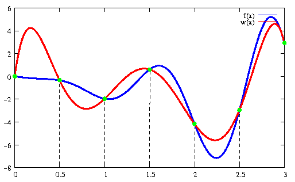
\includegraphics[scale=0.8]{rozdziały/images/Numerki/interpolacja.png}
\end{figure}

\textbf{Twierdzenie}:
Zadanie interpolacji Lagrange'a ma jednoznaczne rozwiązanie.

\textbf{Wyznaczanie WIL}:
\begin{itemize}
    \item w bazie naturalnej, tzn. $w(x)=\sum_ia_ix^i$ mamy
    $$
    \begin{bmatrix}
        1 & x_0 & x_0^2 & \cdots & x_0^N \\
        1 & x_1 & x_1^2 & \cdots & x_1^N \\
        \vdots & \vdots & & \vdots & \\
        1 & x_N & x_N^2 & \cdots & x_N^N
    \end{bmatrix} \cdot \begin{bmatrix}
        a_0 \\
        a_1 \\
        \vdots \\
        a_N
    \end{bmatrix} = \begin{bmatrix}
        f(x_0) \\
        f(x_1) \\
        \vdots \\
        f(x_N)
    \end{bmatrix}
    $$
    Macierz po lewej, zwana macierzą Vandermonde'a, jest gęsta, niesymetryczna, koszt GEPP to $O(N^3)$, a co najgorsze, jest \textbf{patologicznie} źle uwarunkowana! Lepiej wziąć inną bazę.
    \item w bazie Newtona, tzn. $p(x)=\sum_ib_i\cdot(x-x_0)\cdots(x-x_{i-1})$ mamy $b_i=f(x_0,x_1,\ldots,x_i)$, $0\leq i\leq N$, gdzie
    $$
    f(t_0,t_1,\ldots,t_s)=\frac{f(t_1,t_2,\ldots,t_s)-f(t_0,t_1,\ldots,t_{s-1})}{t_s-t_0}
    $$
    to \textbf{różnice dzielone}. Algorytm różnic dzielonych wyznacza WIL \textit{in situ} kosztem $O(N^2)$ flopów.
    $$
    \begin{matrix}
        x_0 & f(x_0) & & & & \\
        x_1 & f(x_1) & f(x_0,x_1) & & & \\
        x_2 & f(x_2) & f(x_1,x_2) & f(x_0,x_1,x_2) & & \\
        \vdots & \vdots & \vdots & \vdots & \ddots & \\
        x_N & f(x_N) & f(x_{N-1},x_N) & f(x_{N-2},x_{N-1},x_N) & \cdots & f(x_0,x_1,\ldots,x_N) \\
    \end{matrix}
    $$
    Powyższą tabelkę wypełniamy kolejnymi kolumnami.
    \item w bazie Lagrange'a, tzn.
    $$
    p(x)=\sum_{i=0}^Na_i\underbrace{\prod_{j\neq i}\frac{x-x_j}{x_i-x_j}}_{=I_i(x)}
    $$
    mamy $p(x)=\sum_{i=0}^N f(x_i)\cdot I_i(x)$, a więc koszt ,,zerowy"! (ale pamiętajmy o koszcie obliczenia wartości $p$ -- istnieje algorytm precomputingu o koszcie $O(N^2)$).
\end{itemize}

\textbf{Twierdzenie (błąd interpolacji)}:
Niech $p$ będzie WIL dla $f$ w punktach $x_0,\ldots,x_N$. Wtedy
\begin{itemize}
    \item dla dowolnego $\overline{x}\in\RR$
    $$
    f(\overline{x})-p(\overline{x})=f(x_0,x_1,\ldots,x_N,\overline{x})\cdot\phi_{N+1}(\overline{x}),
    $$
    \item ponadto, jeśli $f\in C^{(N+1)}[a,b]$, gdzie $[a,b]$ zawiera $x_0,\ldots,x_N,\overline{x}$, to istnieje $\xi=\xi(\overline{x})\in(a,b)$ takie, że
    $$
    f(\overline{x})-p(\overline{x})=\frac{f^{(N+1)}(\xi)}{(N+1)!}\cdot\phi_{N+1}(\overline{x}).
    $$
\end{itemize}
Pamiętamy, że $\phi_{N+1}(x)=(x-x_0)\cdots(x-x_N)$.

\section{Aproksymacja jednostajna}

\subsection{Aproksymacja}
\textbf{PRO8L3M:} Niech $F$ będzie przestrzenią liniowa i niech $V \subset F$ -- podprzestrzeń skończonego wymiaru. Dla danego $f \in F$ znaleźć $v^* \in V$ taki, że
$$
\norm{f - v^*} \leq \norm{f - v} \quad \; \forall v \in V
$$
Mówimy, że $v^*$ jest ENA dla $f$.\\

W przypadku aproksymacji jednostajnej chcemy przybliżyć ciągłą funkcję wielomianami:

Niech:
\begin{itemize}
    \item $F = C[a,b]$ -- przestrzeń funkcji ciągłych

    \item $V = P_N$ -- przestrzeń wielomianów stopnia co najwyżej $N$

    \item $\norm{f}_{\infty} = \sup_{x \in [a,b]} |f(x)|$
\end{itemize}
Wówczas dla zadanej funkcji $f \in C[a,b]$ chcemy znaleźć wielomian $p^* \in P_N$ taki, że
$$
\norm{f-p^*}_{\infty} \to min!
$$

\subsection{Alternans}
Zadajmy zbiór $N+2$ punktów takich, że $a \leq \xi_0 < \xi_1 \ldots < \xi_{N+1} \leq b$. Wówczas alternans to funkcja $e = f - p*$ taka, że
\begin{itemize}
    \item $|e(\xi_i)| = \norm{e}_{\infty} \quad $ dla $i = 0, \ldots, N+1$ 

    \item $e(\xi_i) = -e(\xi_{i+1}) \quad $ dla $i = 0, \ldots, N$ 
\end{itemize}
\textbf{Twierdzenie o alternansie}:

$p* \in P_N$ jest ENA dla $f \iff$ istnieje alternans dla $f$ i $p^*$

\textbf{Węzły Czebyszewa}:
Weźmy $N+1$ węzłów interpolacji $a \leq x_0 < x_1 \ldots < x_{N} \leq b$. Wówczas z twierdzenie na postać błędu interpolacji wiemy, że:
$$
\norm{f-p}_{\infty} \leq \frac{\norm{f^{(N+1)}}_{\infty}}{(N+1)!} \cdot \norm{\phi_{N+1}}_{\infty}
$$
gdzie $\phi_{N+1}(x)=(x-x_0)\cdots(x-x_N)$.

\textbf{PRO8L3M:} Jak dobrać węzły interpolacji tak żeby było jak najbardziej optymalnie?\\

Jeśli $[a,b]=[-1,1]$ to z pomocą przychodzi wybitny ukraiński matematyk Pafnutij Czebyszew. Okazuje się, że najbardziej optymalne węzły to miejsca zerowe wielomianu Czebyszewa $T_{N+1}$ postaci: $$x_i = \cos\left(\frac{2i+1}{2N+2}\pi\right)$$
Co więcej, jeśli $p$ jest WIL opartym na węzłach Czebyszewa to istnieje ograniczenie
$$
\norm{f-p}_{\infty} \leq \frac{\norm{f^{(N+1)}}_{\infty}}{2^N(N+1)!}
$$

\subsection{Metoda bisekcji}
Żeby opisać metodę bisekcji posłużę się słynną interakcją z naszego wydziału:\\


STUDENT: Żaden informatyk nie potrafi bezbłędnie napisać binsearcha od ręki.\\
PCHW: Ja potrafię. \gray{[jebać pchw - przyp. red.]}\\
$[$Pisze binsearcha z błędem$]$

Weźmy sobie $f \in C[a,b]$ taką, że $f(a) \cdot f(b) < 0$. Z twierdzenia Darboux wiemy, że $f$ ma miejsce zerowe w $(a,b)$.

\textbf{PRO8L3M:} Znaleźć miejsce zerowe. \\

Robimy binsearcha.\\
Otrzymujemy $x_n = \frac{1}{2^n}|b-a|$\\
Przy $n$ iteracjach dostajemy ograniczenie
$$
|x_n-x^*| \leq \frac{1}{2^n} |b - a|
$$

\subsection{Szybkość zbieżności metody iteracyjnej}
Ciąg $x_n \to x^* \in \RR^N$ jest: 
\begin{itemize}
    \item zbieżny z rzędem (co najmniej) $p > 1$ jeśli
    $$
    \exists C \geq 0 \quad \norm{x_{n+1}-  x^*}_{\infty} \leq C \norm{x_n - x^*}_{\infty}^p
    $$
    Dla $p=2$ zbieżność kwadratowa, dla $p=3$ kubiczna
    
    \item zbieżny (co najmniej) liniowo jeśli
    $$  
    \exists \gamma \in [0,1) \geq 0 \quad \norm{x_{n+1}-  x^*}_{\infty} \leq \gamma \norm{x_n - x^*}_{\infty}
    $$

    \item $r-$zbieżny z rzędem $p$ (odp. liniowo) jeśli
    $$  
    \norm{x_{n+1}-  x^*}_{\infty} \leq r_n
    $$
    dla pewnego ciągu $r_n$ zbieżnego z rzędem $p$ do 0.\\
    Np. metoda bisekcji jest zbieżna $r-$liniowo z ilorazem $\frac{1}{2}$.
\end{itemize}

\subsection{Punkt stały}
\textbf{PRO8L3M:} Niech $\Phi: D \to R^N$, gdzie $D \subset R^N$. Znajdź $x^*\in D$ taki, że 
$$
x^* = \Phi(x^*)
$$
czyli znajdź punkt stały $\Phi$.\\
Jest to oczywiście równoważny pro8l3m do wyznaczania miejsca zerowego funkcji np.
$$
f(x)= x - \Phi(x)
$$

\textbf{Crème de la crème polskiej matematyki, czyli Twierdzenie Banacha o kontrakcji}:

Niech $\Phi: D \to D$ będzie kontrakcją
$$
\exists L\in[0,1)  \quad \; \norm{\Phi(x) - \Phi(y)} \leq L \norm{x-y}     \quad \forall x,y \in D
$$
Wówczas 

\begin{itemize}
    \item istnieje dokładnie jeden punkt stały $\Phi$

    \item iteracja Banacha
        $$
        x_{n+1} = \Phi(x_n)
        $$
        jest zbieżna liniowo do $x^*$ z dowolnego $x_0 \in D$ 
\end{itemize}

\textbf{Twierdzenie o maszynce rzędu}
Załóżmy, że iteracja $x_{n+1} = \Phi(x_n)$ jest zbieżna do punktu stałego $x^*$, przy czym $\Phi \in C^p(D), p \geq 1$ oraz
$$
\Phi'(x^*) = \cdots = \Phi^{p-1}(x^*)= 0
$$
Jeśli $x_0$ jest dostatecznie blisko $x^*$ to
$$
\exists C \norm{x_{n+1} - x^*} \leq C \norm{x_n-x^*}^p
$$

\subsection{Metoda Newtona}
Niech $f: D \to \RR^n $ oraz $D \subset \RR^N$ otwarty i niepusty. Niech $x^*$ będzie miejscem zerowym $f$. Jeśli
\begin{itemize}
    \item $f$ jest różniczkowalna oraz
    $$
    \exists L \quad \norm{f'(x) - f'(y)} \leq L \norm{x-y}    \quad \forall x,y \in D
    $$
    \item $f'(x^*)$ jest nieosobliwa
\end{itemize}
Iteracja wygląda następująco:\\
$$
x_{n+1} = x_n - \frac{f(x_n)}{f'(x_n)}
$$

to dla $x_0$ dostatecznie blisko (cokolwiek to znaczy) $x^*$ metoda Newtona jest zbieżna kwadratowo.\\
Jeśli dołożymy warunek, że $f''(x^*)=0$ to mamy nawet zbieżność sześcienną

\begin{figure}[H]
    \centering
    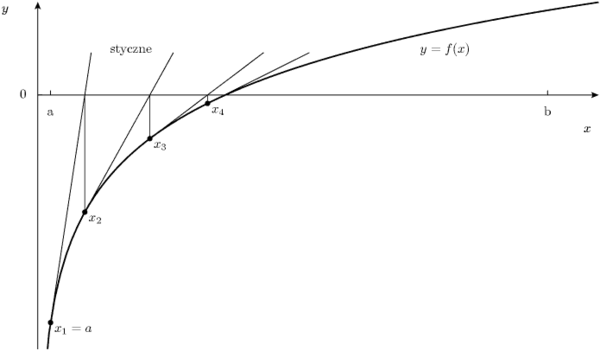
\includegraphics[width=0.75\textwidth]{rozdziały/images/Numerki/600px-Metoda_Newtona-4_kroki.png}
    \caption{Metoda Newtona, pierwsze 4 iteracje}
    \label{fig:enter-label}
\end{figure}


\begin{problems}
    \prob Iteracyjna metoda rozwiązywania równania $f(x) = x - \frac{1}{2(1+x^2)}$ gdzie $x_{n+1} = \frac{1}{2(1+x_n^2)}$, jest
    \answers{zbieżna kwadratowo}{zbieżna dla $x_0=0$}{zbieżna dla $x_0=10$}

    \prob Szukamy zera funkcji $f(x) = x^2 - a$ na przedziale $[0, a]$, używając metody bisekcji. Prawdą jest, że
    \answers{dla $a = 99$ i dziesięciu iteracji błąd znalezionego rozwiązania szacuje się z góry przez $10^{-4}$}{10 iteracji wymaga policzenia co najmniej 20 wartości funkcji}{wzór iteracji dla tej metody to $x_{n+1} = x_n^2 + \frac{a}{2x_n}$}

    \prob Dla danego $a \in \RR$ szukamy rzeczywistych pierwiastków równania nieliniowego $x^3 - x = a$ metodą Newtona. Wówczas
    \answers
    {wzór na kolejną iterację metody to $x_{k+1} = \frac{2x^3_k-a}{3x^2_k+1}$}
    {dla $a = 1$ i dowolnego $x_0 \geq 1$ metoda Newtona jest zbieżna do jakiegoś pierwiastka równania}
    {dla $a = 0$ i $x_0 = 10^{-2}$ metoda Newtona jest zbieżna kwadratowo do zera}
\end{problems}

\section{Metody numeryczne całkowania}

\subsection{Kwadratury}
Będziemy zajmować się następującym \textbf{problemem}:
dla $f:[a,b]\to\RR$ przybliżyć wartość
$$
I(f) = \int_a^b f(x)\rho(x)\ dx
$$
za pomocą kwadratury $\purple{Q(f) = \sum_{i=0}^n A_if(x_i)}$. Chodzi nam o wyznaczenie \textbf{współczynników kwadratury} $A_i$ oraz \textbf{węzłów kwadratury} $x_i\in[a,b]$ takich, by $Q(f)\approx I(f)$ możliwie dobrze w pewnej klasie funkcji $f\in F$.

\textbf{Kwadratury interpolacyjne}:
Idea: funkcję $f$ przybliżyć wielomianem interpolacyjnym $p$, a całkę z $f$ -- całką z $p$. Niech $x_0,\ldots,x_n$ węzły interpolacji Lagrange'a oraz $p(x)=\sum_{i=0}^n f(x_i)\cdot\underbrace{I_i(x)}_{\text{baza Lagrange'a}}$. Wtedy
$$
I(f) \approx Q(f) := \int_a^b p(x)\ dx = \int_a^b \sum_{i=0}^n f(x_i)I_i(x)\ dx = \sum_{i=0}^n\left(\underbrace{\int_a^b I_i(x)\ dx}_{=:A_i}\right)\cdot f(x_i)
$$
$A_i$ -- wyznaczamy raz na zawsze (nie zależą od $f$) w precomputingu: umiemy obliczać całki z wielomianów. Nie wszystkie kwadratury są interpolacyjne.

\textbf{Błąd kwadratur interpolacyjnych}:
Jeśli $f\in C^{n+1}[a,b]$, a $Q$ jest kwadraturą interpolacyjną opartą na węzłach $x_0,\ldots,x_n\in[a,b]$, to
$$
|I(f)-Q(f)| \leq \frac{\norm{f^{(n+1)}}}{(n+1)!}|b-a|^{n+2}.
$$

Istnieje parę prostych kwadratur wymienionych poniżej, wraz z ich błędami:
\begin{itemize}
    \item kwadratura prostokątów:
    $$
    \purple{Q^P(f) = (b-a)\cdot f\left(\frac{a+b}{2}\right)}, \qquad I(f) - Q^P(f) = \frac{(b-a)^3}{24}f''(\xi), \text{ dla pewnego } \xi\in[a,b],
    $$
    \item kwadratura trapezów:
    $$
    \purple{Q^T(f) = \frac{b-a}{2}\cdot(f(a)+f(b))}, \qquad I(f) - Q^T(f) = -\frac{(b-a)^3}{12}f''(\xi), \text{ dla pewnego } \xi\in[a,b],
    $$
    \item kwadratura parabol (Simpsona):
    $$
   \purple{ Q^S(f) = \frac{b-a}{6}\cdot\left(f(a)+4f\left(\frac{a+b}{2}\right)+f(b)\right)}, \quad I(f) - Q^S(f) = -\frac{(b-a)^5}{2880}f^{(4)}(\xi), \text{ dla pewnego } \xi\in[a,b].
    $$
\end{itemize}

Kwadratura $Q$ dla całki $I(f) = \int_a^b f(x)\rho(x)\ dx$ jest rzędu (co najmniej) $r$, jeśli
$$
\forall_{p\in P_{r-1}} I(p)=Q(p).
$$
Jest \textbf{rzędu} $r$, gdy jest co najmniej rzędu $r$, ale już nie $r+1$.

\textbf{Wniosek}:
Każda kwadratura interpolacyjna oparta na $n$ węzłach jest co najmniej rzędu $n$.

\textbf{Twierdzenie}:
Rząd kwadratury interpolacyjnej opartej na $n$ węzłach nie przekracza $2n$. Realizuje go kwadratura Gaussa, oparta na zerach $n$-tego wielomianu ortogonalnego w $L_\rho^2(a,b)$.

\begin{problems}
    \prob Całkę $\int_{-1}^{1} f(x)$ przybliżamy kwadraturą interpolacyjną $Q(f) = A_1f(x_1)+A_2f(x_2)$. Wtedy
    \answers{dla $A_1=A_2 = 1$, $x_1= -1$, $x_2 = 1$ kwadratura $Q$ jest dokładna dla wszystkich wielomianów stopnia $1$}{można dobrać $x_1$ i $x_2$, tak aby kwadratura $Q$ była rzędu $2$ oraz $A_1=A_2=2$}{maksymalny rząd kwadratury $Q$ jest równy $4$}

    \prob Stosując metodę złożonej kwadratury trapezów na odcinku $[a, b]$ dla funkcji $f$, można obliczyć dokładnie (pomijając błędy zaokrągleń) całkę $\int_{a}^{b} f(x) \dx$ dla
    \answers{$f(x) = 3 - x$}{$f(x) = 3 - x + x^2$}{$f(x) = \sin(x)$}
\end{problems}

\begin{solutions}
    \sol $A$ jest macierzą nieosobliwą $N \times N$. Wynika z tego, że
    \answerss
    {istnieją macierze $L$ dolnotrójkątna i $U$ górnotrójkątna $N \times N$, takie że $A = LU$}
    {istnieją macierz permutacji $Q$ oraz macierze $L$ dolnotrójkątna i $U$ górnotrójkątna $N \times N$, takie że $AQ = LU$}
    {istnieją macierz permutacji $P$ oraz macierze $L$ dolnotrójkątna i $U$ górnotrójkątna $N \times N$, takie że $PA = LU$}
    {TAK}{TAK}{TAK}
    Na macierzy nieosobliwej działa klasyczny algorytm podziału $LU$ bez wyboru elementu głównego. Dlatego \textbf{A.} to prawda. W szczególności macierzą permutacji $Q$ w drugim podpunkcie może być macierz identycznościowa. Wtedy faktycznie $AQ=AI=A=LU$, więc \textbf{B.} \texttt{TAK}. Ten podpunkt był jednak podchwytliwy, gdyż przy algorytmie z wyborem elementu głównego otrzymujemy $PA=LU$, a nie $AP=LU$ (a przynajmniej zawsze tak pisał Przykry). Ponieważ działa algorytm bez GEPP, to zadziała $P=I$, ale przy wyborze elementu głównego może się faktycznie coś pozmieniać i wtedy $P$ będzie jakieś inne, ale też w porządku. Stąd \textbf{C.} jest git.
    
    \sol $A$ jest macierzą nieosobliwą o wymiarach $N\times N$. Wynika z tego, że koszt wyznaczenia macierzy $A^{-1}$
    \answerss{za pomocą algorytmu $LU$ wynosi $O(N^2)$ operacji arytmetycznych}{wynosi $O(N^2)$ operacji arytmetycznych, jeśli $A$ jest górnotrójkątna}{wynosi $O(1)$ operacji arytmetycznych, jeśli $A$ jest macierzą Householdera}{NIE}{NIE}{TAK}
    \textbf{A.} Uzyskanie rozkładu $LU$ już zajmuje czas $O(N^3)$. \\
    \textbf{B.} Zajmuje czas $O(N^3)$, chociaż układ $Rx=y$ możemy rozwiązać w $O(N^2)$. Znając $x$ i mając $R^{-1}Rx=Ix=x=R^{-1}y$ widać, że tak łatwo tego nie obliczymy -- może być $O(N^3)$ elementów. A tak po prostacku odwracać macierz to radzę nawet nie próbować. \\
    \textbf{C.} Macierz Householdera jest swoją własną odwrotnością.

    % Grześ
    \sol Mamy daną macierz $A = \begin{bmatrix}
        7 & -13 & 16\\
        -13 & 10 & -13\\
        16 & -13 & 7 \\
    \end{bmatrix}$
    oraz wektor $x_0 = \begin{bmatrix}
        2019 \\
        2020 \\
        2021 
    \end{bmatrix}$. Niech $y_n = A x_{n}$ oraz $ x_{n+1} = \frac{y_{n}}{\norm{y_{n}}}$. Wtedy
    \answerss{$\Lim_{k \to \infty} \norm{x_k} = 1$}{$\Lim_{k \to \infty} \frac{x_{k}^T A x_{k}}{x_{k}^T x_{k}} = 1$}{ciąg $\{x_n\}_{n \geq 0}$ jest zbieżny}{TAK}{NIE}{TAK}
    \textbf{A.} Zauważmy, że $x_{n+1}=\frac{y_n}{\norm{y_n}}=\frac{Ax_n}{\norm{Ax_n}}$, czyli z każdą iteracją normalizujemy wektor, tj. skracamy/wydłużamy go, aby miał długość 1, czyli ta granica już po pierwszej iteracji jest prawdziwa.

    \textbf{B.} Wiedząc, że $x_k\to v$, gdzie $v$ jest wektorem własnym macierzy $A$ mamy
    $$
    \Lim_{k\to\infty}\frac{x_{k}^T A x_{k}}{x_{k}^T x_{k}} = \Lim_{k\to\infty}\frac{v^T A v}{v^T v} = \lambda\Lim_{k\to\infty}\frac{v^T v}{v^T v} = \lambda = 1.
    $$
    Pytanie, czy 1 jest wartością własną macierzy $A$? Aby to sprawdzić, rozwiązujemy układ równań $Av=v$, czyli dla $v=[x_1,x_2,x_3]^T$:
    $$
    \begin{cases}
        7x_1 - 13x_2 + 16x_3 = x_1 \\
        -13x_1 + 10x_2 - 13x_3 = x_2 \\
        16x_1 - 13x_2 + 7x_3 = x_3
    \end{cases}
    $$
    co zostawiam jako zadanie dla Czytelnika.

    \textbf{C.} Tak, patrząc na wzór z podpunktu \textbf{A.} widzimy, że jest to metoda potęgowa, która jest zbieżna do wektora/wartości własnej macierzy $A$.

    % Patryk
    \sol Iteracyjna metoda rozwiązywania równania $f(x) = x - \frac{1}{2(1+x^2)}$ gdzie $x_{n+1} = \frac{1}{2(1+x_n^2)}$, jest
    \answerss{zbieżna kwadratowo}{zbieżna dla $x_0=0$}{zbieżna dla $x_0=10$}{NIE}{TAK}{TAK}
    
    Trzeba zauważyć że funkcja $\Phi(x) = \frac{1}{2(1+x^2)}$ to kontrakcja (jak to zauważyć? ~ trudno). Wówczas z twierdzenia Banacha o kontrakcji wiemy, że \textbf{B.} i \textbf{C.} jest prawdą. Użyjmy maszynki do rzędu żeby ocenić szybkość zbieżności tej metody. Pochodna $\Phi'(x) = \frac{-x}{(1+x^2)^2}$ ma miejsce zerowe dla $x_0 = 0$, a to na pewno nie jest punkt stały, więc metoda jest zbieżna liniowo.

    % Patryk
    \sol Szukamy zera funkcji $f(x) = x^2 - a$ na przedziale $[0, a]$, używając metody bisekcji. Prawdą jest, że
    \answerss{dla $a = 99$ i dziesięciu iteracji błąd znalezionego rozwiązania szacuje się z góry przez $10^{-4}$}{10 iteracji wymaga policzenia co najmniej 20 wartości funkcji}{wzór iteracji dla tej metody to $x_{n+1} = x_n^2 + \frac{a}{2x_n}$}{NIE}{NIE}{NIE}
    
    \textbf{A.} Błąd ten szacuje się z góry przez $\frac{1}{2^{10}}\cdot99 \approx 0.1$.

    \textbf{B.} Wymaga tylko 10.

    \textbf{C.}Taki ciąg nie oddaje idei metody bisekcji. Dla $x>0$ ten ciąg jest rosnący, co nie ma sensu z punktu widzenia bisekcji.

    % Grześ
    \sol Dla danego $a \in \RR$ szukamy rzeczywistych pierwiastków równania nieliniowego $x^3 - x = a$ metodą Newtona. Wówczas
    \answerss
    {wzór na kolejną iterację metody to $x_{k+1} = \frac{2x^3_k-a}{3x^2_k+1}$}
    {dla $a = 1$ i dowolnego $x_0 \geq 1$ metoda Newtona jest zbieżna do jakiegoś pierwiastka równania}
    {dla $a = 0$ i $x_0 = 10^{-2}$ metoda Newtona jest zbieżna kwadratowo do zera}
    {NIE}{TAK}{TAK}
    \textbf{A.} Szukamy miejsca zerowego funkcji $f(x)=x^3-x-a$, która jest różniczkowalna, a jej pochodna to $f'(x)=3x^2-1$. Wówczas, wzór na kolejną iterację tej metody to
    $$
    x_{k+1} = x_k - \frac{f(x_k)}{f'(x_k)} = x_k - \frac{x_k^3-x_k-a}{3x_k^2-1} = \frac{3x_k^3-x_k-x_k^3+x_k+a}{3x_k^2-1} = \frac{2x_k^3+a}{3x_k^2-1},
    $$
    co wygląda podobnie, ale to nie jest $\frac{2x_k^3-a}{3x_k^2+1}$.

    \textbf{B.} Mamy $f(x)=x^3-x-1$ i $f'(x)=3x^2-1$. Szybko zauważymy, że w punkcie $x=\frac{1}{\sqrt{3}}$ funkcja $f$ osiąga minimum lokalne, a rozwiązanie $x^*\in(1,2)$ z własności Darboux. Ponadto, dla $x>\frac{1}{\sqrt{3}}$ funkcja już cały czas rośnie do nieskończoności, więc startując z dowolnego punktu $x_0>\frac{1}{\sqrt{3}}$ na pewno metoda zbiegnie kwadratowo do miejsca zerowego $x^*$.

    \textbf{C.} Szukamy miejsca zerowego $f(x)=x^3-x=x(x-1)(x+1)$. Startując z $x_0=10^{-2}$ jesteśmy bardzo blisko 0 i najprawdopodobniej metoda Newtona zbiegnie kwadratowo właśnie do 0, ale nawet jak coś się wydarzy niespodziewanego, zbiegnie tak czy siak do $-1$ lub 1.

    \sol Całkę $\int_{-1}^{1} f(x)$ przybliżamy kwadraturą interpolacyjną $Q(f) = A_1f(x_1)+A_2f(x_2)$. Wtedy
    \answerss{dla $A_1=A_2 = 1$, $x_1= -1$, $x_2 = 1$ kwadratura $Q$ jest dokładna dla wszystkich wielomianów stopnia $1$}{można dobrać $x_1$ i $x_2$, tak aby kwadratura $Q$ była rzędu $2$ oraz $A_1=A_2=2$}{maksymalny rząd kwadratury $Q$ jest równy $4$}{TAK}{NIE}{TAK}
    \textbf{A.} Niech $p(x)=ax+b$. Wtedy $\int_{-1}^1 p(x)\ dx=(\frac{a}{2}x^2+bx)\big|_{-1}^1=(\frac{a}{2}+b)-(\frac{a}{2}-b)=2b$, a kwadratura wynosi $Q(f)=A_1f(x_1)+A_2f(x_2)=(a+b)+(-a+b)=2b$, więc jest dokładna.

    \textbf{B.} \texttt{NIE}, bo jak wiemy z poprzedniego podpunktu, $\int_{-1}^1p(x)\ dx=2b$, a taka kwadratura $Q$ wynosi $Q(f)=2(ax_1+b)+2(ax_2+b)=2a(x_1+x_2)+4b$, więc nawet jakbyśmy wzięli $x_1=-x_2$, to nie pozbędziemy się nadmiarowych $2b$.

    \textbf{C.} Wynika to wprost z twierdzenia o rzędzie.

    \sol Stosując metodę złożonej kwadratury trapezów na odcinku $[a, b]$ dla funkcji $f$, można obliczyć dokładnie (pomijając błędy zaokrągleń) całkę $\int_{a}^{b} f(x) \dx$ dla
    \answerss{$f(x) = 3 - x$}{$f(x) = 3 - x + x^2$}{$f(x) = \sin(x)$}{TAK}{NIE}{NIE}
    \textbf{A.} $\int_a^b(3-x)\ dx=(3x-\frac{x^2}{2})\big|_a^b=(3b-\frac{b^2}{2})-(3a-\frac{a^2}{2})=\frac{a^2-b^2}{2}+3(b-a)=\frac{b-a}{2}(6-a-b)$, \\
    $Q^T(f)=\frac{b-a}{2}(3-a+3-b)=\frac{b-a}{2}(6-a-b)$, więc odpowiedź to \texttt{TAK}.

    \textbf{B.} $\int_a^b(3-x+x^2)\ dx=(3x-\frac{x^2}{2}+\frac{x^3}{3})\big|_a^b=(3b-\frac{b^2}{2}+\frac{b^3}{3})-(3a-\frac{a^2}{2}+\frac{a^3}{3})=\frac{b^3-a^3}{3}+\frac{a^2-b^2}{2}+3(b-a)=\frac{b-a}{2}(6-a-b+\frac{2(a^b+ab+b^2)}{3})$, \\
    $O^T(f)=\frac{b-a}{2}(3-a+a^2+3-b+b^2)=\frac{b-a}{2}(6-a-b+a^b+b^2)$, więc odpowiedź to \texttt{NIE}.

    \textbf{C.} Aż żal to liczyć, widać, że $I(f)\neq Q^T(f)$.
\end{solutions}
